\section{\gls{fdtd} simulation} \label{sec:fdtd_simulation}
The aim of this chapter is to make a simulation of the zero order gradient speaker, first order gradient speaker and the solution proposed in \autoref{sec:opt_result} using \gls{fdtd}. All simulation cross all three different method of using speaker at low frequency will be compared in both free field and inside a room. The result will be discussed with respect to directionality and efficiency. 

\section{\gls{fdtd} step size}
This section will determined the the step size for both grid size and the time step size. As the time step size is depending on the grid step size, the grid step size will be determined first. Recalling \autoref{fdtd_delta_stepsize} state that all three dimention will have the same step size in this project, the calculation is as following \autoref{fdtd_distance_stepsize} 

\begin{subequations}\label{fdtd_distance_stepsize}
\begin{alignat}{2}
d &= \delta x = \delta y = \delta z \leq \frac{1}{10} \frac{c}{f_{max}} \label{fdtd_distance_stepsize_1}\\
d &= \frac{1}{10} \frac{\SI{343}{\meter\per\second}}{\SI{300}{\hertz}} \label{fdtd_distance_stepsize_2}\\
d &= \SI{0.11}{\meter} \label{fdtd_distance_stepsize_3}
\end{alignat}
\end{subequations}

    \startexplain
    		\explain{$d$ is the maximum grid cell size }{\si{\meter}}
        \explain{$c$ is the speed of sound at 20 degree}{\si{\meter\per\second}}
        \explain{$f_{max}$ is the maximum frequency in the simulation}{\si{\hertz}}
    \stopexplain

Since the maximum grid cell size is \SI{11}{\centi\meter}, the grid cell size is in this project will be less or equal to \SI{10}{\centi\meter}, to be sure that a simulation does not suffer from a limiting grid cell size. \\

From the optimization \autoref{sec:opt_result} it is determined that the optimal distance between the side speaker is \SI{50}{\centi\meter} and to the front speaker it is \SI{30}{\centi\meter}. The greatest common divisor is \SI{5}{\centi\meter} which then is the grid step size in all simulation. Next the time step have to be determined. The condition for time step is staded in \autoref{fdtd_time_stepsize_boundary} and gives following \autoref{fdtd_time_stepsize_con_one}
    
 
    \begin{subequations}\label{fdtd_time_stepsize_con_one}
\begin{alignat}{2}
\delta t &\leq \sqrt{\frac{2}{3}}  \left( \frac{1}{\sqrt{\frac{1}{(\delta x)^2}+\frac{1}{(\delta x)^2}+\frac{1}{(\delta x)^2} }\cdot c} \right)\\
\delta t &\leq \sqrt{\frac{2}{3}}  \left( \frac{1}{\sqrt{\frac{1}{(\SI{0.05}{\meter})^2}+\frac{1}{(\SI{0.05}{\meter})^2}+\frac{1}{(\SI{0.05}{\meter})^2} }\cdot \SI{343}{\meter\per\second}} \right)\\
\delta t &\leq \SI{687}{\micro\second} 
\end{alignat}
\end{subequations}
    
 Which correspond to a sampling frequency of at least \SI{14552}{\hertz}, and  to be sure that a simulation does not suffer from a limiting time step size, the time step size will be rounded up to \SI{14560}{\hertz}.
 
 
The time step have to be small enough such that standard walls can be included in the simulation, and since plaster wall is well used, $Z_{1}$ is possible nonzero and therefore both condition in \autoref{sec:fdtd_time_stepsize} has to be satisfied. 
 
 The second condition is \autoref{fdtd_time_stepsize_boundary_Z_n1} where plaster is chosen as the limit case for soft walls and concrete is chosen as the limit for hard walls. The calculation for plaster walls is as following \autoref{fdtd_time_stepsize_con_plaster} \citep{finiteproblems}.
 
     \begin{subequations}\label{fdtd_time_stepsize_con_plaster}
\begin{alignat}{2}
c \delta t &\leq \delta x \left(   \frac{1+\frac{2Z_1}{\rho_0 \delta x}}{1+\frac{2Z_{-1} \delta x}{\rho_0 c^2}}  \right)^{\frac{1}{2}}\\
 \delta t &\leq \frac{\SI{0.10}{\meter} \left(   \frac{1+\frac{2\cdot 6}{1.21 \cdot \SI{0.10}{\meter}}}{1+\frac{2 \cdot 16 \cdot \SI{0.10}{\meter}}{1.21 \cdot {343}^2}}  \right)^{\frac{1}{2}}}{343}\\
\delta t &\leq \SI{2.92}{\milli\second} 
\end{alignat}
\end{subequations}
 Which correspond to a sampling frequency of at least \SI{343}{\hertz}.


concrete is missing??


It can be concluded that the grid step size $d$ shall be \SI{100}{\milli\meter} and the sampling frequency $\frac{1}{\delta t}$ shall at least be equal or higher than \SI{7399}{\hertz}, The impulse response from the used \gls{dut} will be used as the impulse response in all simulation. All impulse response measurement in this project have a sample frequency of \SI{44.1}{\kilo\hertz} but because the simulation does not have to have higher sample frequency than \SI{7399}{\hertz}, the sample frequency of the measurement will be down sampled with a factor of 6. The choose of a factor of 6 is justified by that this is the highest scalar factor the measurement sampling frequency can be down sampled  and still satisfy the minimum sampling frequency and also keeping the required process power down. This result in a sampling frequency for the simulation of \SI{7.35}{\kilo\hertz}

\section{\gls{fdtd} implementation}
The aim of this section is to convert the grid to matrices. Since the grid is in three dimension where the time is the fourth dimension, the whole matrix system for pressure and all particle velocity matrices will built on four dimensional matrices. The following \autoref{fig:fdtd_cartesian_grid} shows a simple grid in a corner with entry notation of $h$ as the hight of the room, $w$ as the width of the room and $l$ as the length of the room.


\begin{figure}[H]
	\centering
\begin{picture}(0,0)%
\includegraphics{fdtd_grid_matrices.pdf}%
\end{picture}%
\setlength{\unitlength}{4144sp}%
%
\begingroup\makeatletter\ifx\SetFigFont\undefined%
\gdef\SetFigFont#1#2#3#4#5{%
  \reset@font\fontsize{#1}{#2pt}%
  \fontfamily{#3}\fontseries{#4}\fontshape{#5}%
  \selectfont}%
\fi\endgroup%
\begin{picture}(3869,4070)(3541,-1873)
\put(5941,1334){\color[rgb]{0,0,1}$v_x(2,1,1)$}%
\put(4186,434){\color[rgb]{0,0,0}$(l,w,h)$}%
\put(5041,1019){\color[rgb]{0,0,1}$v_x(1,1,1)$}%
\put(6211,974){\color[rgb]{0,.82,0}$v_y(1,2,1)$}%
\put(5941,1604){\color[rgb]{.82,0,0}$v_z(1,1,1)$}%
\put(5041,749){\color[rgb]{.82,0,0}$v_z(1,1,2)$}%
\put(4771,1379){\color[rgb]{0,.82,0}$v_y(1,1,1)$}%
\put(5491, 74){\color[rgb]{1,0,0}$p(1,1,2)$}%
\put(6931,1199){\color[rgb]{1,0,0}$p(2,1,1)$}%
\put(6391,569){\color[rgb]{1,0,0}$p(1,2,1)$}%
\put(4996,-376){Pressure point}%
\put(4996,-736){Unknown pressure point}%
\put(3556,1244){$z$}%
\put(4996,-1096){Particle velocity x-direction}%
\put(4996,-1456){Particle velocity y-direction}%
\put(4006,704){$x$}%
\put(3826,344){$y$}%
\put(4996,-1771){Particle velocity z-direction}%
\end{picture}%
	\caption{The figure visualized a boundary plan through particle velocity plan $x$ in 1 dimension}
		\label{fig:fdtd_cartesian_grid}
\end{figure}

All simulation is done i MATLAB and therefore the $x$ direction is implemented as matrix rows direction and $y$ direction is implemented as matrix column direction. The hight $h$ is implemented as the third dimension and the time is implemented as the fourth dimension. The particle velocity will be calculated as the first step and the pressure will be calculated as the second step. The time dimension is only as small as 2 page, because it is only necessary to save at $l-1$ and at $l$. All time further away than $l-1$ is not used in the calculation and will be deleted for keeping the needed storage as low as possible. 

\subsection{\gls{fdtd} boundary}
The particle velocity at the boundary in all direction have to be calculated as in \autoref{fdtd_boundary_result} and this is done as a step between the particle velocity matrices and the pressure matrices. This mean for the particle velocity in $x$ direction the first and last matrix row is calculated by the boundary formula and in $y$ direction the first column and the last matrix column is calculated by the boundary formula. 


\section{\gls{fdtd} plot}
The aim of the section is to explain how the resulting phase, gain and distance from \autoref{ch:optimization} is implemented in a \gls{fdtd} simulation, and how the result of the simulation is compared with the polar plot from \autoref{ch:optimization}. \\

To be able to simulate the result from \autoref{ch:optimization} three pressure point is used as the acoustical center. The pressure point is implemented as transparent point sources, where all the point sources is fed with a sinusoid of a single frequency where the phase and gain is adjusted to the specified frequency. The Front speaker will always be feeded with a gain of one, which correspond to a pressure of $\pm \SI{1}{\pascal}$ and zero phase. Therefore it is only the back speaker which will be adjusted phase and gain wise. The simulation run step is the smallest room size divided by the grid size, such that the wave do not reflect from the wall. \\

A wave will expand in a circular form and since the simulation stops just before the it hits the first wall, The simulation will be a circular shape. Some of the area is not simulated and is therefore pressure less. The simulation is therefore made so large that the polar plot with a radius of \SI{10}{\meter} still can be calculated, where the used simulation data is only a squared area inside the circular shape and the rest data is discarded. The following figures compares the analytical model with the simulated model. 


\begin{figure}[H]
\centering
\begin{subfigure}[htbp]{0.55\textwidth}
		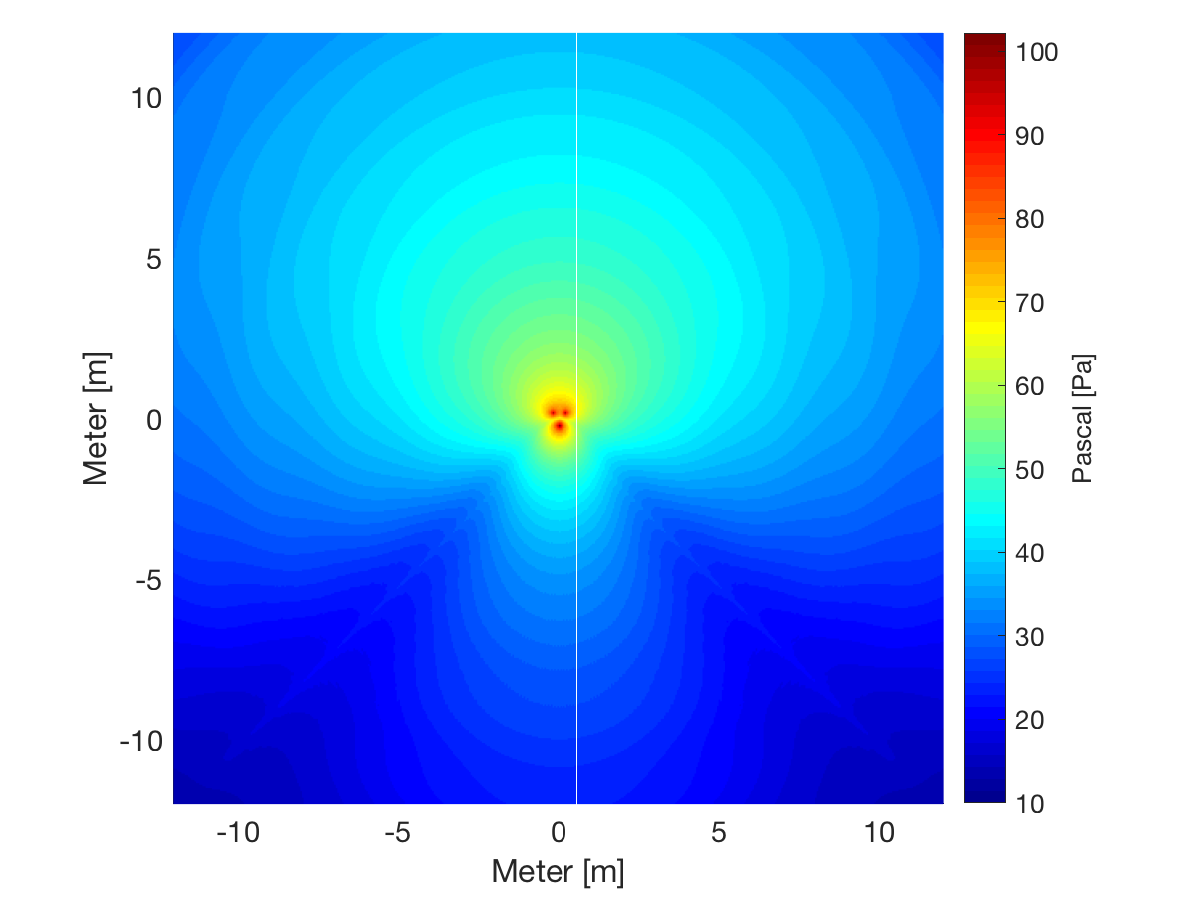
\includegraphics[width=\textwidth]{60_hz_fdtd_plot}
		\caption{The figure shows the \gls{fdtd} simulation of \SI{60}{\hertz}}
		\label{fig:fdtd_60_Hz}
\end{subfigure}
\begin{subfigure}[htbp]{0.35\textwidth}
		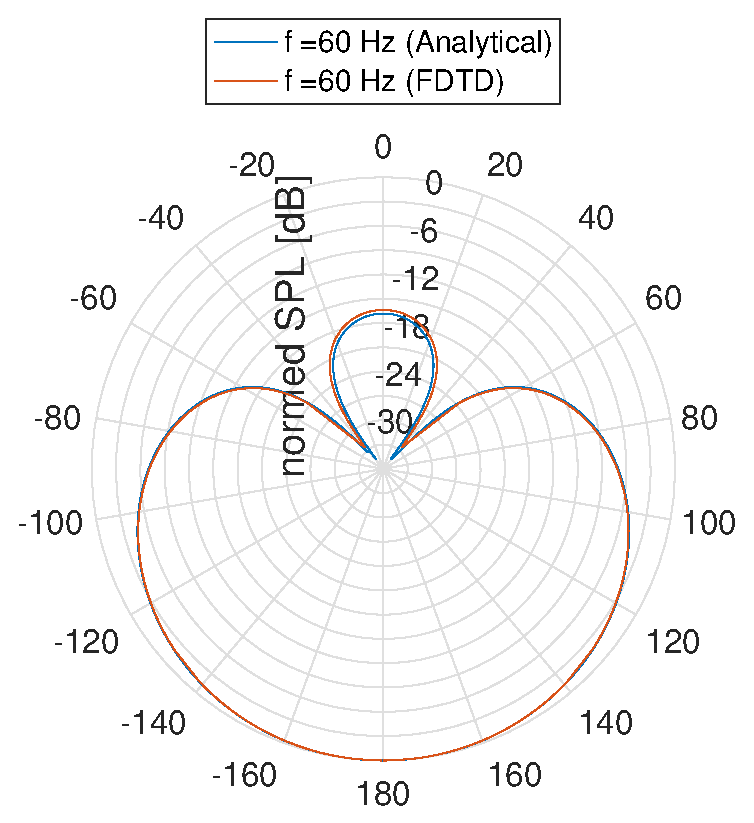
\includegraphics[width=\textwidth]{60_hz_polar_plot}
		\caption{The figure shows the analytical- and \gls{fdtd} polar plot at \SI{60}{\hertz} with a radius of \SI{10}{\meter}}
		\label{fig:polar_60_Hz}
\end{subfigure} 
\caption{The figure compares the analytical model and the \gls{fdtd} model of the cardioid speaker model at \SI{60}{\hertz}}
\end{figure}


\begin{figure}[H]
\centering
\begin{subfigure}[htbp]{0.55\textwidth}
		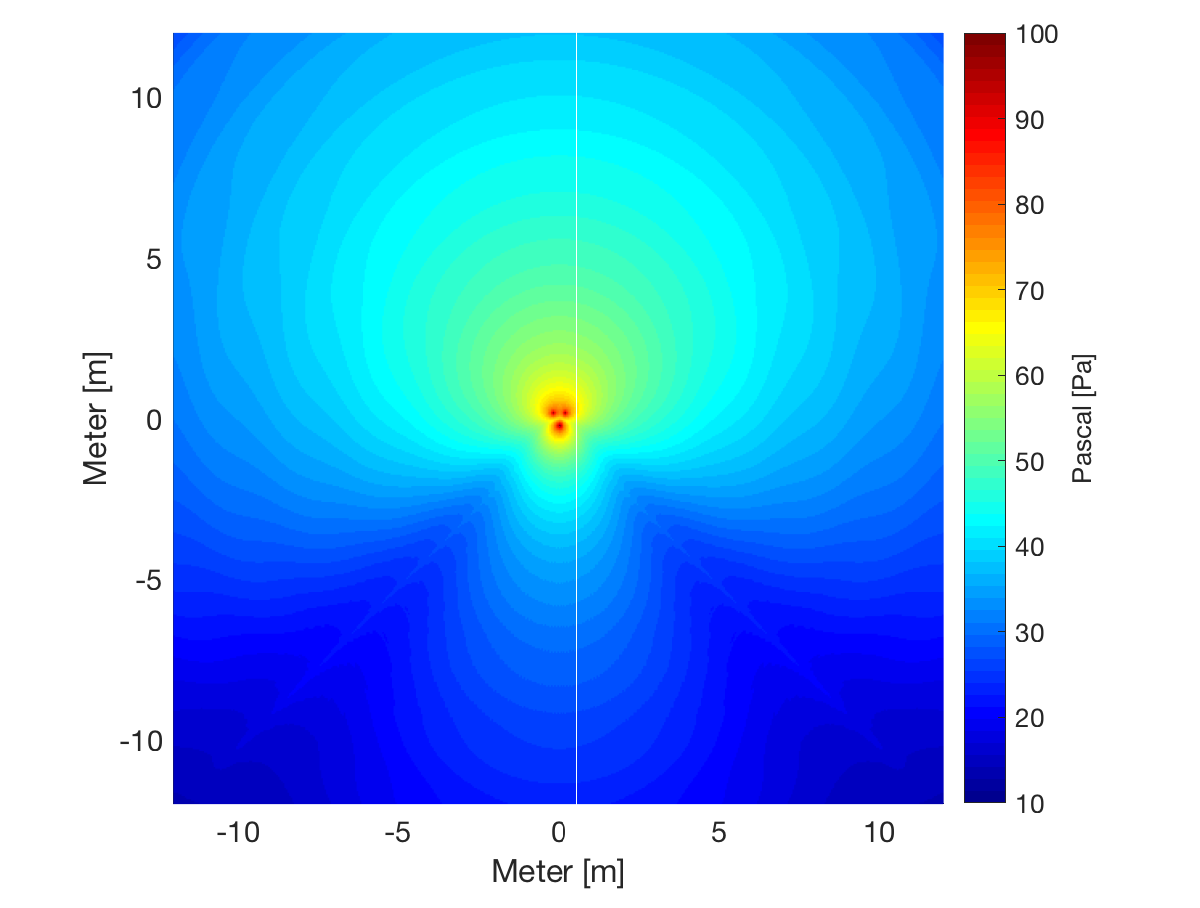
\includegraphics[width=\textwidth]{70_hz_fdtd_plot}
		\caption{The figure shows the \gls{fdtd} simulation of \SI{70}{\hertz}}
		\label{fig:fdtd_70_Hz}
\end{subfigure}
\begin{subfigure}[htbp]{0.35\textwidth}
		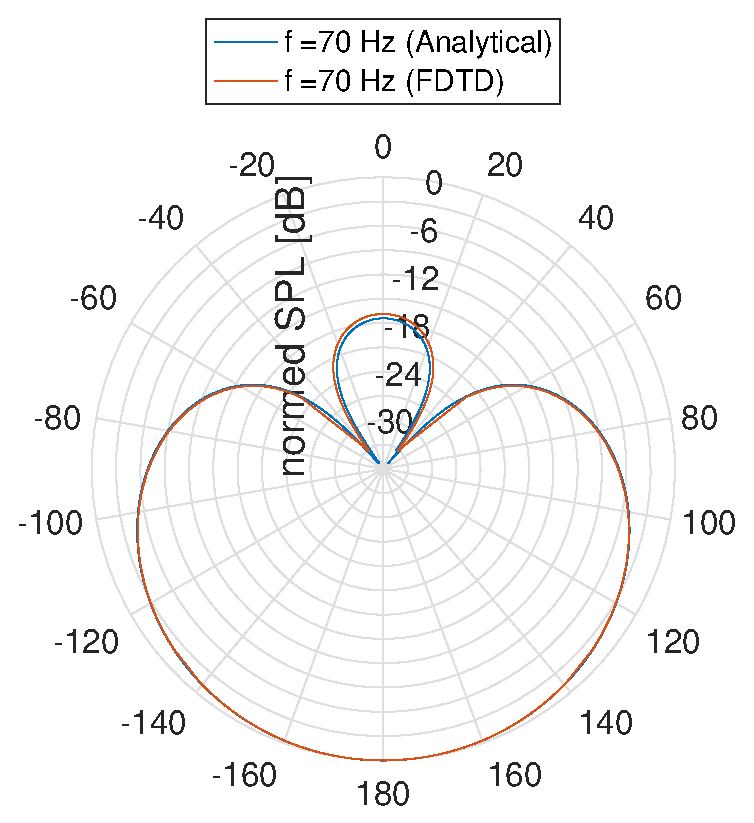
\includegraphics[width=\textwidth]{70_hz_polar_plot}
		\caption{The figure shows the analytical- and \gls{fdtd} polar plot at \SI{70}{\hertz} with a radius of \SI{10}{\meter}}
		\label{fig:polar_70_Hz}
\end{subfigure} 
\caption{The figure compares the analytical model and the \gls{fdtd} model of the cardioid speaker model at \SI{70}{\hertz}}
\end{figure}


\begin{figure}[H]
\centering
\begin{subfigure}[htbp]{0.55\textwidth}
		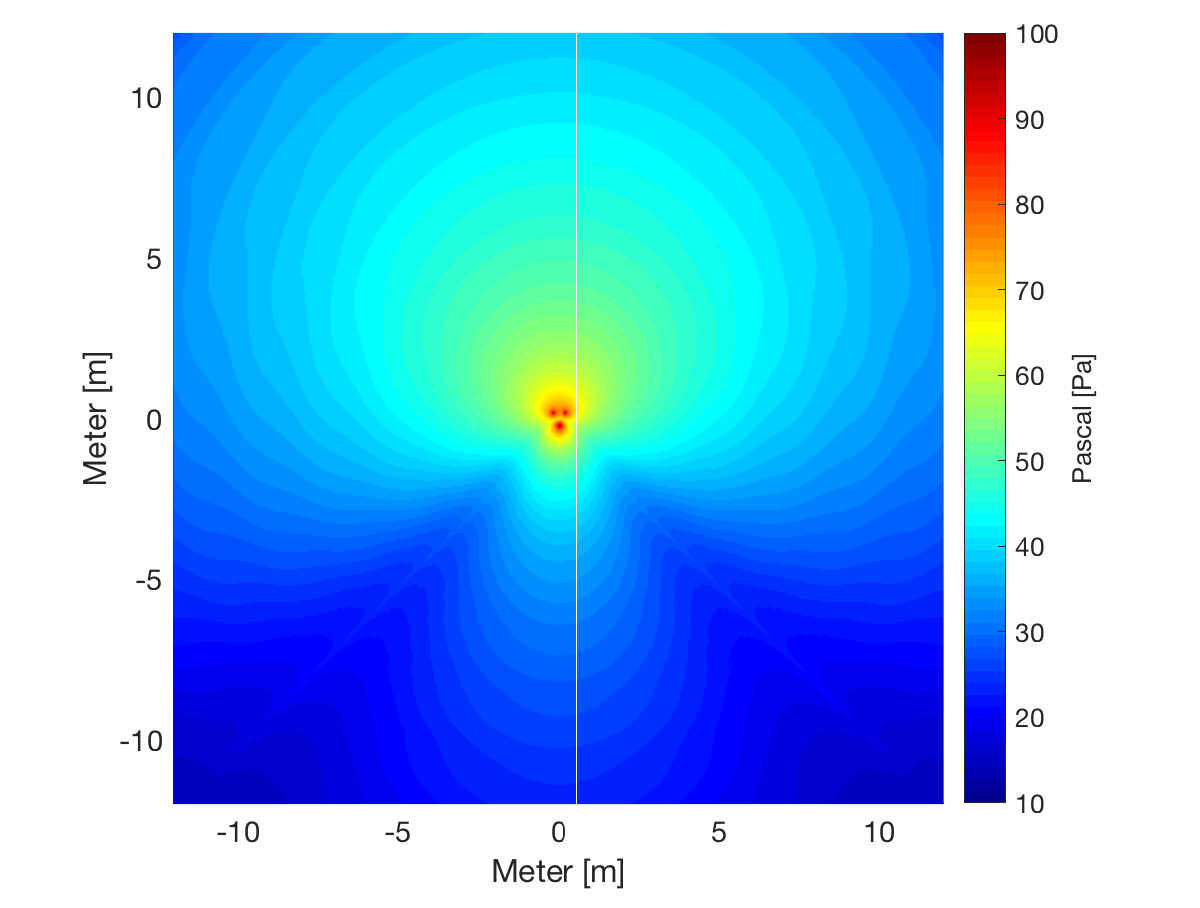
\includegraphics[width=\textwidth]{80_hz_fdtd_plot}
		\caption{The figure shows the \gls{fdtd} simulation of \SI{80}{\hertz}}
		\label{fig:fdtd_80_Hz}
\end{subfigure}
\begin{subfigure}[htbp]{0.35\textwidth}
		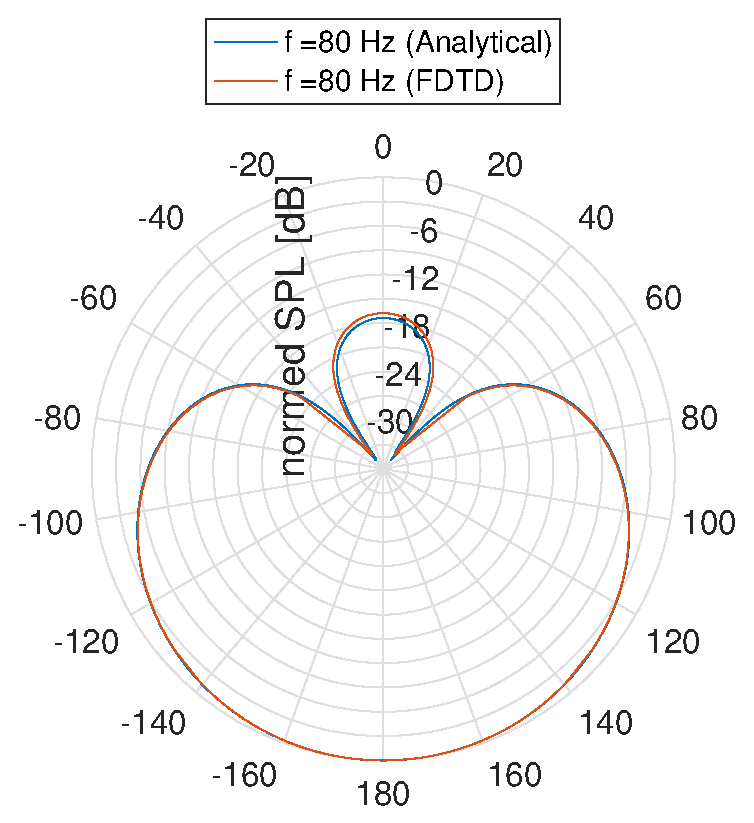
\includegraphics[width=\textwidth]{80_hz_polar_plot}
		\caption{The figure shows the analytical- and \gls{fdtd} polar plot at \SI{80}{\hertz} with a radius of \SI{10}{\meter}}
		\label{fig:polar_80_Hz}
\end{subfigure} 
\caption{The figure compares the analytical model and the \gls{fdtd} model of the cardioid speaker model at \SI{80}{\hertz}}
\end{figure}


\begin{figure}[H]
\centering
\begin{subfigure}[htbp]{0.55\textwidth}
		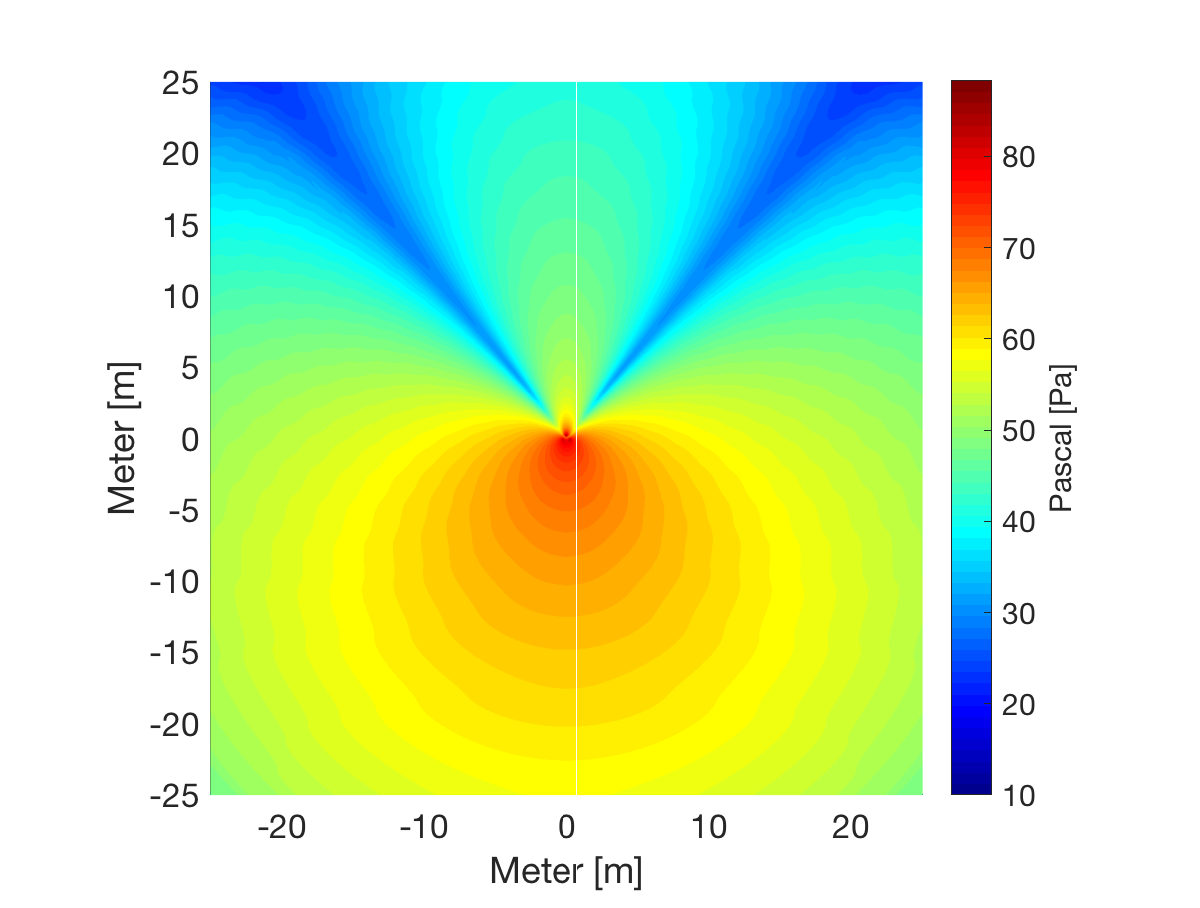
\includegraphics[width=\textwidth]{90_hz_fdtd_plot}
		\caption{The figure shows the \gls{fdtd} simulation of \SI{90}{\hertz}}
		\label{fig:fdtd_90_Hz}
\end{subfigure}
\begin{subfigure}[htbp]{0.35\textwidth}
		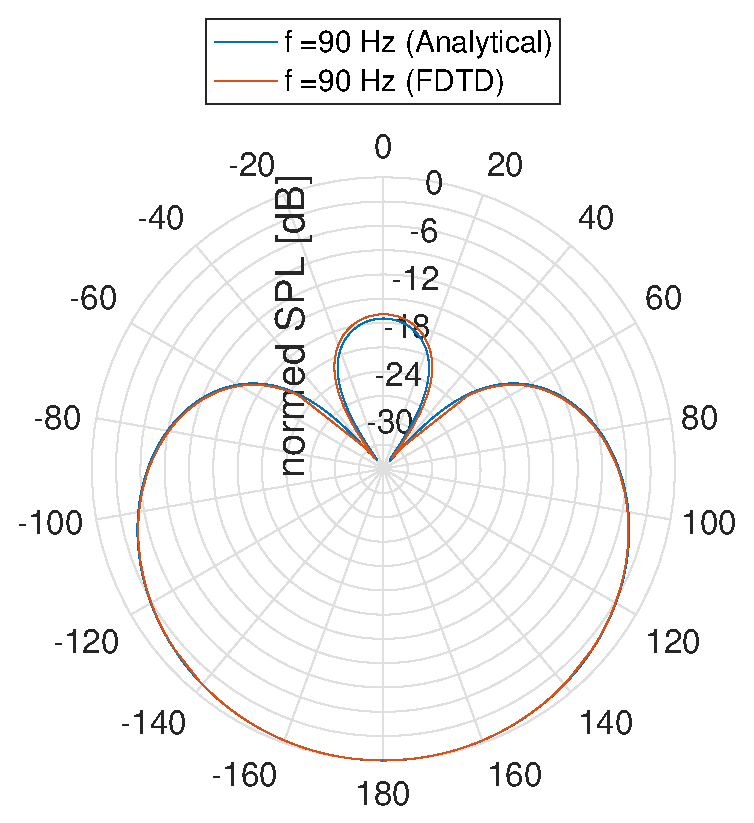
\includegraphics[width=\textwidth]{90_hz_polar_plot}
		\caption{The figure shows the analytical- and \gls{fdtd} polar plot at \SI{90}{\hertz} with a radius of \SI{10}{\meter}}
		\label{fig:polar_90_Hz}
\end{subfigure} 
\caption{The figure compares the analytical model and the \gls{fdtd} model of the cardioid speaker model at \SI{90}{\hertz}}
\end{figure}


\begin{figure}[H]
\centering
\begin{subfigure}[htbp]{0.55\textwidth}
		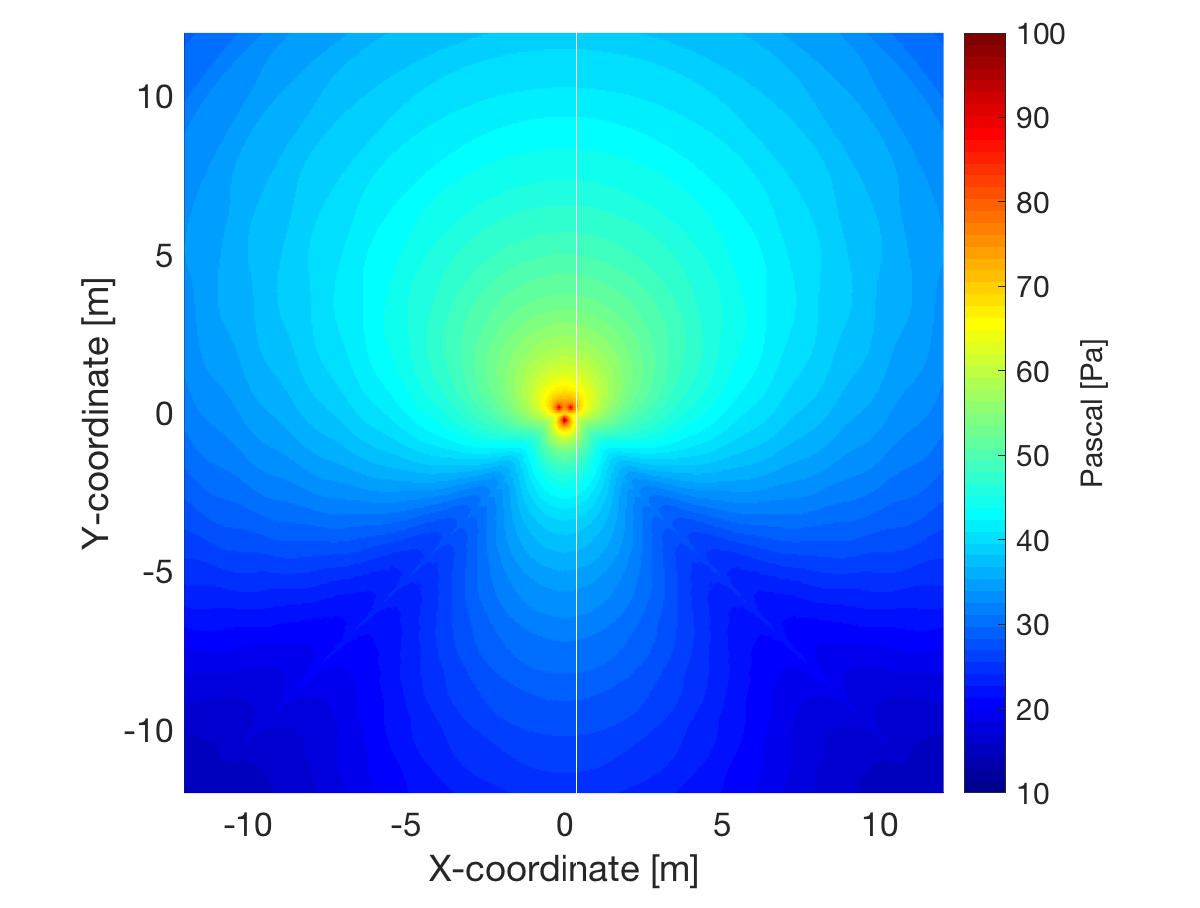
\includegraphics[width=\textwidth]{100_hz_fdtd_plot}
		\caption{The figure shows the \gls{fdtd} simulation of \SI{100}{\hertz}}
		\label{fig:fdtd_100_Hz}
\end{subfigure}
\begin{subfigure}[htbp]{0.35\textwidth}
		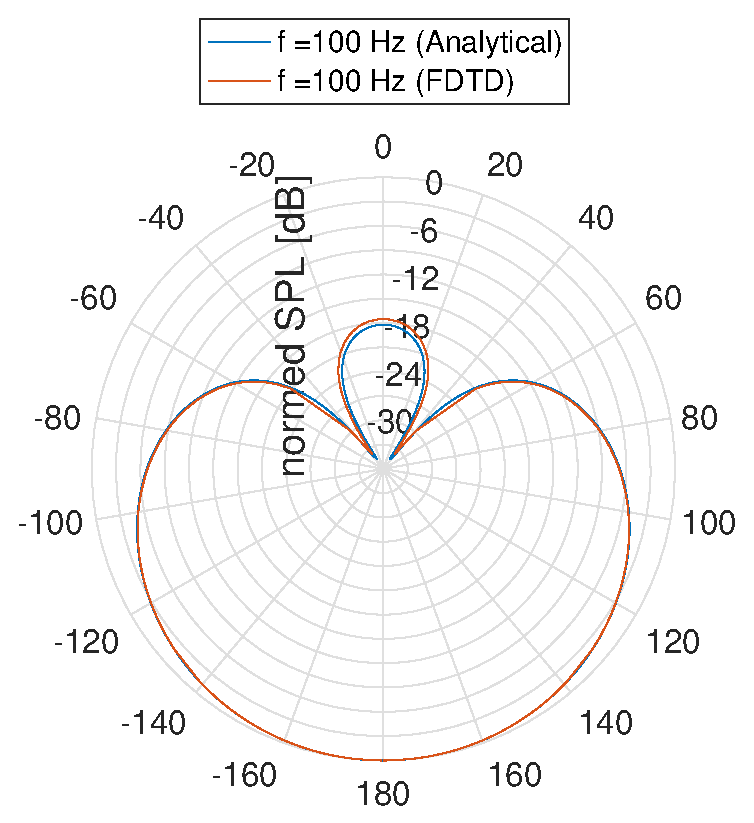
\includegraphics[width=\textwidth]{100_hz_polar_plot}
		\caption{The figure shows the analytical- and \gls{fdtd} polar plot at \SI{100}{\hertz} with a radius of \SI{10}{\meter}}
		\label{fig:polar_100_Hz}
\end{subfigure} 
\caption{The figure compares the analytical model and the \gls{fdtd} model of the cardioid speaker model at \SI{100}{\hertz}}
\end{figure}

\section{Conclusion}